\chapter{Planning de travail}
\label{annexe:planning}

Lors des premières semaines de travail, nous avons établi un planning de travail (voir figure~\ref{fig:plan}), celui-ci a été construit de manière logique, en partant des idées les plus larges et en allant vers les tâches les plus concrète. On voit très bien l'évolution en escalier au fil des semaines.

\begin{figure}	
\begin{center}
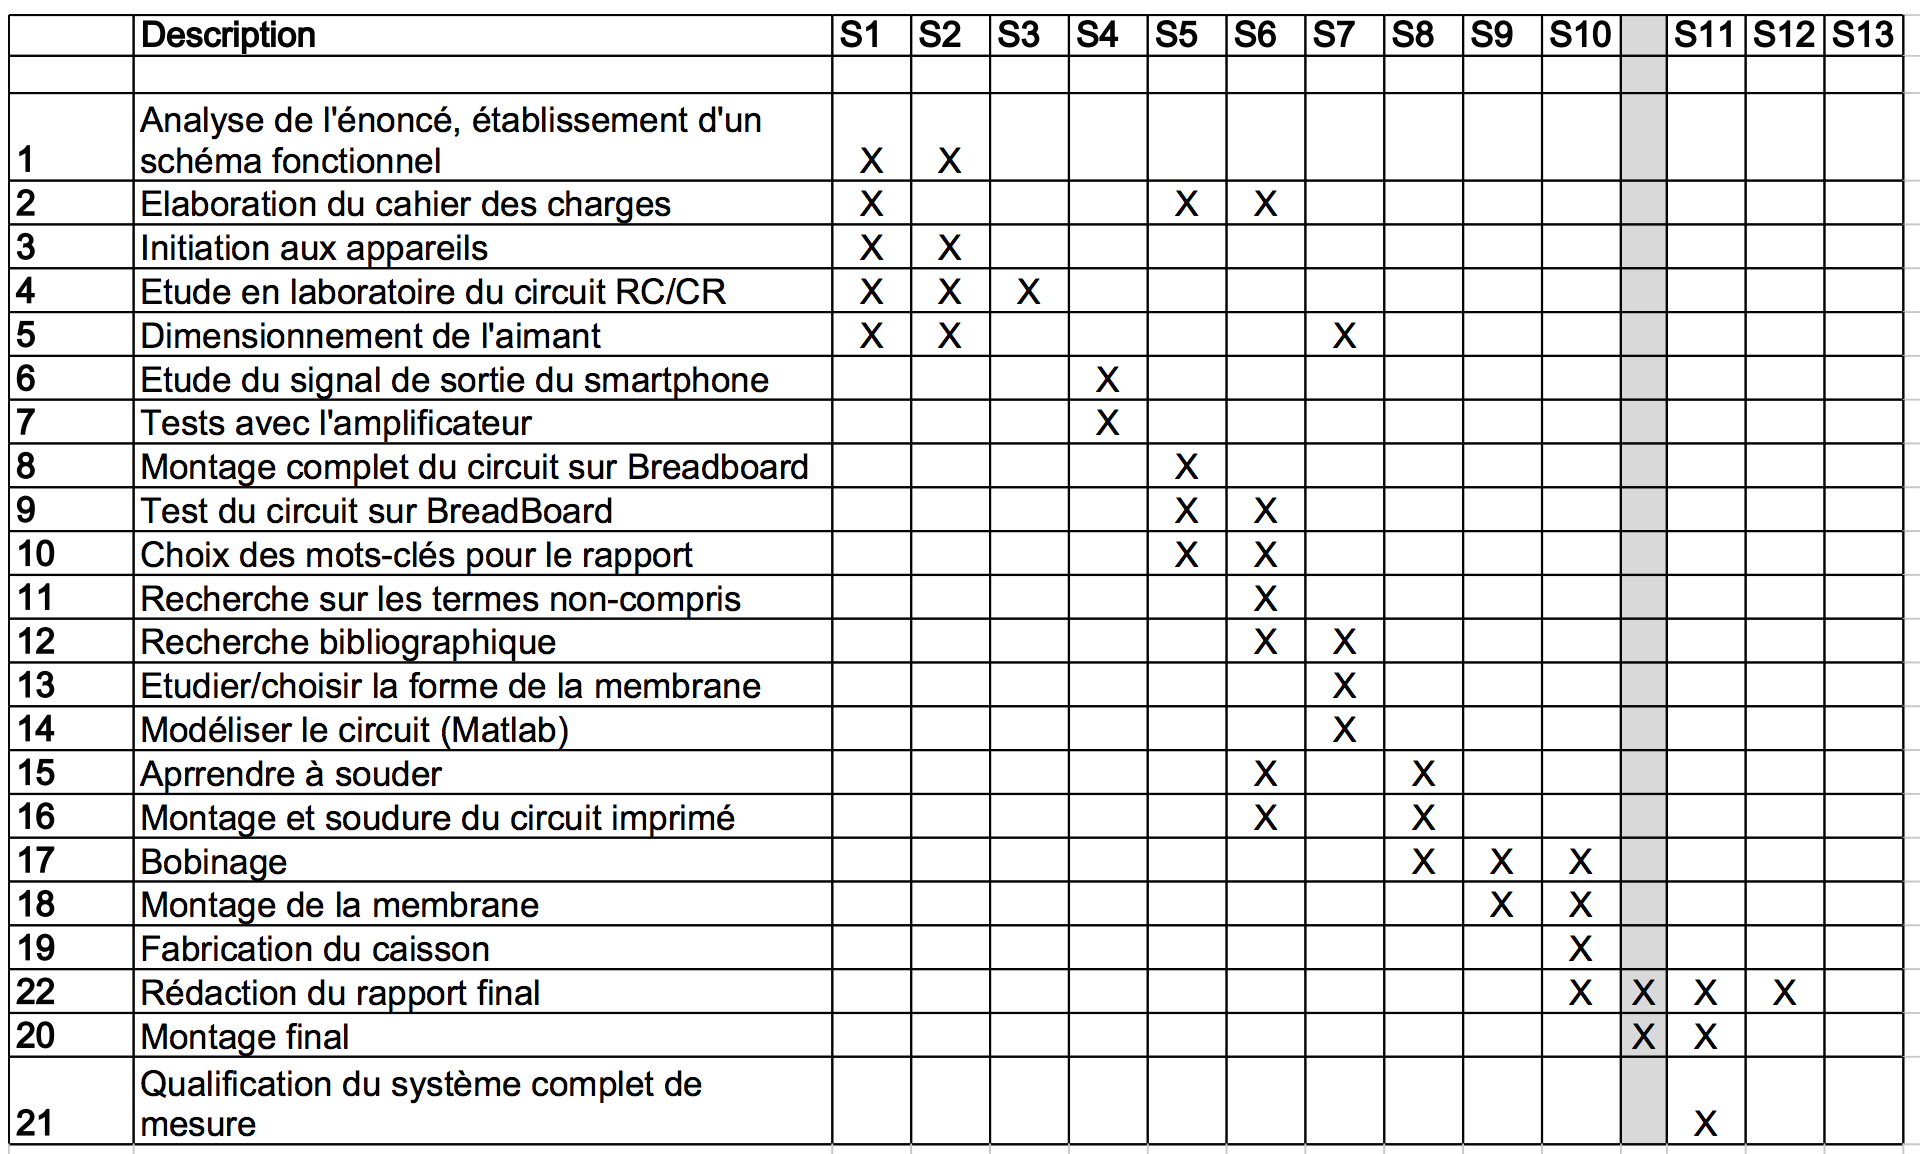
\includegraphics[width=\textwidth]{img/planning} 
\end{center}
\caption{Planning de travail}		
\label{fig:plan}		
\end{figure}

Tout d'abord, il nous a fallu analyser l'énoncé afin de créer un cahier des charges qui correspondait le mieux à ce qui nous était demandé et aux contraintes qui nous étaient imposées. 
En parallèle, au laboratoire, nous avons appris à utiliser les appareils de mesure du laboratoire et nos premières études ce sont portées sur le fonctionnement des circuits CR/RC.

Ensuite, nous avons pu entrer dans le vif du sujet avec le dimensionnement de l'électroaimant, l'étude du signal de sortie du smartphone et le montage de circuit sur breadboard.

Après divers tests, nous avons appris à souder afin de monter le circuit sur la PCB. En parallèle, nous avons commencé la recherche documentaire, point essentiel à la compréhension de notre système.

A l'approche des vacances de Pâques, ils nous a fallut effectuer les bobinages ainsi que réaliser les caissons et les membranes pour notre haut-parleur. Nous avons à ce moment là pu déjà effectuer les premiers tests sur le système complet.

Enfin, les derniers points qui restaient à aborder étaient la rédaction du rapport final, le montage final de notre haut-parleur et la qualification du système de mesure complet de celui-ci.

